\begin{frame}{The Browser RTC Function}

\begin{columns}
\column{.5\textwidth}
\begin{itemize}
\item New Browser Real-Time Communication (RTC) Function built-in to browsers
\item Contains
\begin{itemize}
\item Audio and video codecs
\item Ability to negotiate peer-to-peer connections
\item Echo cancellation, packet loss concealment
\end{itemize}
\item In Chrome and Mozilla today
\end{itemize}
\column{.5\textwidth}
\begin{figure}
\includegraphics[page=2,width=\textwidth]{image/webrtc.pdf}
\end{figure}
\end{columns}

\end{frame}

\begin{frame}{So What's the Big Deal}
\begin{itemize}
\item The web is now a platform for real-time communications development
\item Communication will be secure (encrypted) by default
\item Latest audio and video codecs means superior quality to anything else
\item WebRTC provides peer-to-peer media, even through NATs
\item Standard that can interoperate with existing VoIP, video conferencing, and even PSTN
\end{itemize}
\end{frame}

\begin{frame}{WebRTC Triangle}
\begin{figure}
\includegraphics[page=3,width=.6\textwidth]{image/webrtc.pdf}
\end{figure}
\begin{itemize}
\item Both browsers running the smae web application from web server
\item Peer Connection media session is establised between them
\item Signaling is not standardized, could be SIP, Jingle, proprietary. Uses HTTP or WebSockets for transport
\end{itemize}
\end{frame}

\begin{frame}{WebRTC Trapezoid}
\begin{figure}
\includegraphics[page=4,width=.6\textwidth]{image/webrtc.pdf}
\end{figure}
\begin{itemize}
\item Similar to SIP Trapezoid
\item Web Servers communicatie using SIP or Jingle
\item Useful for building conventional telephony apps, but unclear how this works in the web world
\end{itemize}
\end{frame}

\begin{frame}{WebRTC and SIP}
\begin{figure}
\includegraphics[page=5,width=.6\textwidth]{image/webrtc.pdf}
\end{figure}
\begin{itemize}
\item Peer Connection appears as a standard RTP media session, described by SDP
\item Web Server implements a JSEP (JavaScript Session Establishment Protocol) to SIP signaling gateway
\item SIP Endpoint must support RTCWEB Media extensions (ICE NAT Traversal, Secure RTP, etc.)
\end{itemize}
\end{frame}

\begin{frame}{WebRTC with SIP}
\begin{figure}
\includegraphics[page=6,width=.6\textwidth]{image/webrtc.pdf}
\end{figure}
\begin{itemize}
\item Browser runs a SIP User Agent by running JavaScript form Web Server
\item Secure RTP media connection uses WebRTC APIs
\item Details in [draft-ietf-sipcore-websocket] that defines SIP transport over WebSockets
\end{itemize}
\end{frame}

\begin{frame}{WebRTC and PSTN}
\begin{figure}
\includegraphics[page=7,width=.6\textwidth]{image/webrtc.pdf}
\end{figure}
\begin{itemize}
\item Peer Connection terminates ona PSTN Gateway
\item Audio only
\item Could also use SIP trunking such as SIPconnect 1.1 recommendation
\end{itemize}
\end{frame}

\begin{frame}{WebRTC Support fo Multiple Media}
\begin{figure}
\includegraphics[page=8,width=.6\textwidth]{image/webrtc.pdf}
\end{figure}
\begin{itemize}
\item Multiple sources of audio and video are assumed and supported
\item All RTP media, voice and video, and RTCP feedback messages are multiplexed over the same UDP port and address
\end{itemize}
\end{frame}